\chapter{Introduction}
\label{sec:introduction}
% Overall introduction to the problem. 
% Discuss very early lots of data, not lots of labeling, and no straightforward way to ameliorate this
% Include plots of a few different types of precipitation
% Rob had 2 pages here
Weather radars in the United States produce a vast amount of data every year.
This data is invaluable to researchers in many fields, including atmospheric science, meteorology, and weather radar engineering.
The data represents many types of phenomena in the atmosphere, and is critically important in forewarning disasters and in characterization of the atmospheric effects that relate directly to public safety, agriculture, and recreation.

Weather radar data is also extremely expensive to produce, maintain, and analyze.
Development of research radars is a task few groups in few universities are equipped to attempt, as it requires a start-up cost not only in the millions of dollars, but also in terms of the wide-ranging human capital and expertise needed to develop these sophisticated, high-fidelity instruments.
Additionally, simply managing the data is a complicated task, involving large amounts of compute power to turn complex time series returns into human-readable radar variables and visualize them in real-time.
There is also a need for simply storing the data, necessitating costly servers with huge data footprints.

Given the immense amount of expertise and cost in producing, analyzing, and storing this data, it is perhaps surprising that so little is known about the data after it has been stored.
Research groups embark upon years-long projects that culminate in seasons-long field campaigns, transporting radars domestically and internationally, and involving tens to hundreds of professionals to collect critically important data, but there remains no satisfactory method or set of methods for semantic tagging of the data once it has been collected, beyond radar technicians on the ground noting events as they occur.

Efforts have begun to move data from the WSR-88D radars in the NEXRAD system in the US to cloud storage, reducing the overhead in providing data to researchers, and simplifying said researchers' access to the data.
Simultaneously, projects are in development to leverage cloud compute to help reduce Time to Science in utilizing this and other datasets, along with simplifying the programming overhead to allow scientists to analyze their data using techniques and services in modern infrastructure.
The data available in the cloud, along with that present data silos at various universities and national labs in the United States, encodes priceless insights and a multitude of opportunities for researchers to leverage, should they be able to access it.

\section{Problem Statement}
\label{sec:introduction_problem}
% Rob's pointed out the importance of wind turbines and radar, and stressed that each need to continue living in the same spaces
% Discussed briefly how certain techniques could be used to remove certain types of signatures in wind turbines
% Rob had 2 pages here as well

With respect to weather radar data, there is no simple way to query the large amounts of data available to researchers in a semantic search.
Text-based data has been the focus of search engines which have illustrated methods for extracting valuable information for the past twenty years. 
Natural images, such as photographs, have been studied for decades, and recent developments in deep learning continue to increase the semantic information available in image data.
There may be ways to apply these insights to weather radar data as well, as it is generally stored and presented as images.

Similarly to natural images, in fact, the amount of radar data produced and easily available to researchers and engineers continues to grow at a high rate.
The radar network perhaps most well known to researchers is the NEXRAD network, which is comprised of over 150 dual-polarimetric S-band WSR-88D weather radars observing the atmosphere at all times, located throughout the United States.
An upper estimate of the data produced in a day by a typical WSR-88D, assuming a 1 degree beamwidth, no beam overlap, 460 range gates per radial, could be given by

\begin{equation}
\frac{6 \mathrm{scans}}{\mathrm{hr}} \cdot \frac{24 \mathrm{hr}}{\mathrm{day}} \cdot 360 \mathrm{radials} \cdot \frac{460 \mathrm{gates}}{\mathrm{radial}} \cdot \frac{6 \mathrm{vars}}{\mathrm{scan}} \cdot \frac{12 \mathrm{elevations}}{\mathrm{VCP}} \cdot \frac{4 \mathrm{bytes}}{\mathrm{pixel}} = 6.9 \mathrm{GB}
\end{equation}

where $\mathrm{VCP}$ stands for the volume coverage pattern, and $6 \mathrm{sars}$ refers to 6 radar variables.
This is considered an upper estimate since it assumes a data point in every pixel at every elevation angle, which is rarely the case, but it drives home the point that weather radars are producing a lot of data every day.
Furthermore, considering all 160 WSR-88D radars, scanning every day for a year, an upper estimate on data produced annually is 401 TB. 
This is an extremely large dataset, and represents more data than humans can tractably parse in a meaningful manner.
When we consider that this is only data from one radar network in the United States, and that similar networks are operating in Europe (Opera) and China, there is a sense of urgency around developing modern technological methods for extracting information from and labeling these voluminous datasets, in real-time and on historical data.

\begin{figure}[h]
	\centering
	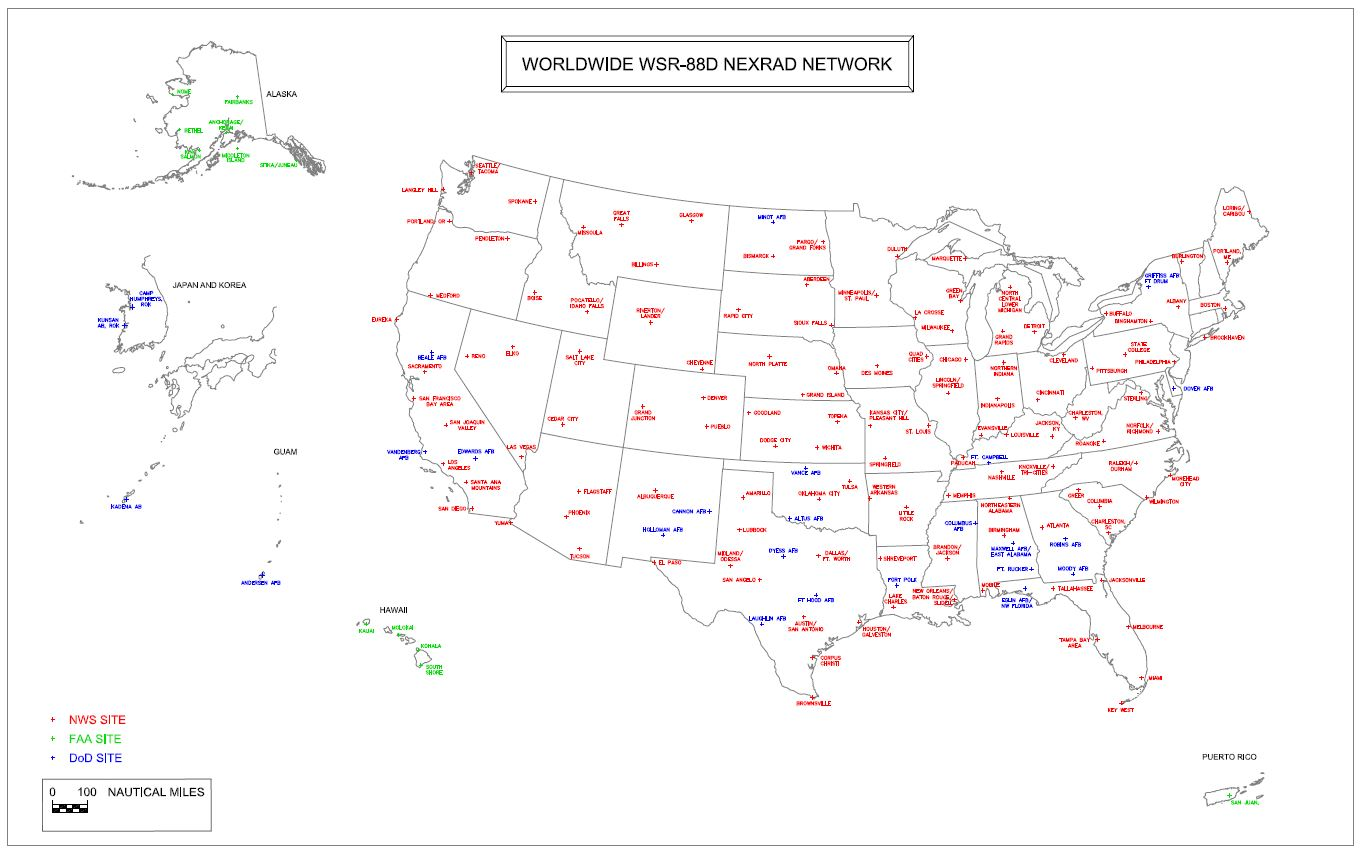
\includegraphics[width=\textwidth]{./thesis_code/plots/noaa_wsr88d_map.jpg}
	\caption{WSR-88D radar sites in the US and abroad. Image can be found at \url{https://www.roc.noaa.gov/WSR88D/Maps.aspx}}
	\label{fig:introduction_wsr88d-map}
\end{figure}

As such, it is urgent and appropriate to explore methods of analyzing the algorithms that have provided such insights in the natural image domain, and using techniques designed in the computer vision sub-field of transfer learning, attempt to extract information in weather radar image data.

\section{Research Objectives}
\label{sec:introduction_objectives}
% Rob: "This dissertation proposal aims to characterize wind turbine clutter with a focus on the dual-polarization signature of wind turbines in the presence of precipitation and ground clutter."
% First sentence is thesis statement after setting everything up

This dissertation proposal aims to develop an automated method for characterizing the spatial information available in weather radar scan data, utilizing information present in dual-polarimetric radar variables.
The long-term goal of this research proposal is to develop a set of automated methods to classify precipitation regimes and to illustrate the feasibility of deploying these models on voluminous weather radar datasets to extract insights and populate semantic tags to facilitate Data Discovery.
This proposal also aims to demonstrate that information available in natural image datasets and the models trained upon these datasets can transfer learning to the domain of weather radar data, allowing researchers to develop their own tools and locate specific atmospheric phenomena of interest by following the techniques presented herein.

Hand-labeling can and must be employed to generate an initial dataset for training the target task, image classification of precipitation regimes.
Once this is completed, techniques from the computer vision sub-field of Transfer Learning can be used to train models to learn functions to perform this classification.
The optimal models above can be determined via theoretical and empirical testing using readily available benchmarked datasets.
An iterative process can be then embarked upon to deploy the model on new data to perform classifications and increase dataset size.
Using a combination of automated classification and hand-labeling of the new generated data, a satisfactorily large dataset can be generated to train new models and finalize learning.

The key points to be addressed in this research are:
\begin{itemize}
	\item Hand-labeling weather radar data to produce a dataset for initially training models
	\item Determining optimal end-to-end deep learning architectures for learning and classifying similar images from benchmark datasets
	\item Using radar reflectivity image data from a research radar network to perform precipitation regime image classification
	\item Demonstrating the encoding of multiple radar variables into three-channel images to enhance classification ability
	\item Deployment of learned models on unseen data available in research radar network to automate data discovery and further enhance dataset, ultimately producing a hand- and machine-labeled dataset to supply to other researchers
	\item Employing the model on the national network of weather radars in the NEXRAD system, thus demonstrating effectiveness of the model at multiple spatial resolutions and radar frequencies
	\item Utilizing tools like CHORDS to perform semantic image classification in real-time
\end{itemize}

\section{Proposal Overview}
\label{sec:introduction_overview}
% Discuss what's in the following sections in the proposal

Chapter \ref{sec:background} presents a review of necessary and relevant literature for this research, with a focus on previously developed methods in weather radar image analysis, as well as transfer learning. 
Additionally, some background information on the calculation of various radar variables is presented, with specific focus on relevant radar moments in this work and how they are visualized both in real-time, and stored on disk.
Finally, the weather radar networks examined in this research are discussed.

Chapter \ref{sec:meteorology} discusses the meteorological phenomena that can be seen in weather radar data, and how they present in the images as functions of radar variables.
Precipitation regimes are examined, with some atmospheric precursors and products discussed to explore the relevance of these patterns and why they should be the foci of this classification work.
The spatial and temporal characteristics of the radar returns are discussed within the scope of how they are viewed in the radar data, so as to better understand the textures and patterns that the deep learning architectures will learn to classify.

Chapter \ref{sec:classifying} details the experiments performed to select and train the deep learning models.
Initially there is a treatment of relevant concepts and math used in machine learning, to develop the nomenclature and standards that follow.
Both shallow and deep networks are discussed in brief as necessary.
An experiment is performed to select a convolutional base and illustrate the utility of using large models in transfer learning tasks.
A set of experiments designed to illustrate the learning ability of the selected convolutional base and top model are detailed, utilizing a readily available benchmark dataset called MNIST-Fashion, chosen to mirror both natural images as well as weather radar images.
Next, the target task of weather radar images are classified according to their corresponding precipitation regimes, using hand-labeled data from a radar in the CASA DFW Urban Testbed of X-band weather radars.
Finally, relevant concerns are detailed regarding the proposed research of deploying models on data from the rest of the CASA DFW network, using multi-channel data with multiple radar variables to produce pseudo-images that encode greater amounts of information for training and testing, and deploying models on the S-band WSR-88D NEXRAD radars.

Chapter \ref{sec:bestmodel} describes the effect of using the model obtained in \ref{sec:classifying} to classify images from two months in 2018 to increase dataset size, as well as the effect of applying new layer technologies to the deep learning architecture.
A new optimal model is discovered, trained, and then deployed on unseen data from 2019, and a brief statistical and climatological examination is performed based on these classifications.

Chapter \ref{sec:realtime} discusses advances in real-time weather radar data, and details the research in implementing weather radar data as a core component of the Cloud-HOsted Real-Time data Services in the geosciences (CHORDS) portal.
This chapter details a survey of current methods in real-time weather radar data visualization, along with modern cyberinfrastructure concerns related to the storage and visualization of weather radar data.
The current CF/Radial standard is discussed, as well as the importance in using such standards to promote findability, accessibility, interoperability, and reusability (FAIR) principles in the domain of weather radar data.

Chapter \ref{sec:summary} summarizes the findings in this research project, and outlines a few potential new avenues that have been opened up as a result of this work.

The Appendix \ref{sec:appendix-a-tools} discusses certain practical considerations for deep learning research and their use in this work.

